This is the delete course page accessible by the professor.\\
The professor can only delete courses that he/she has created.\\
To find the course to delete, he can either search for it through the search bar, or he can browse through all of his courses by hand.\\
Once the course is found, to delete it simply click on the related blue box.\\

\begin{figure}[H]
    \centering
     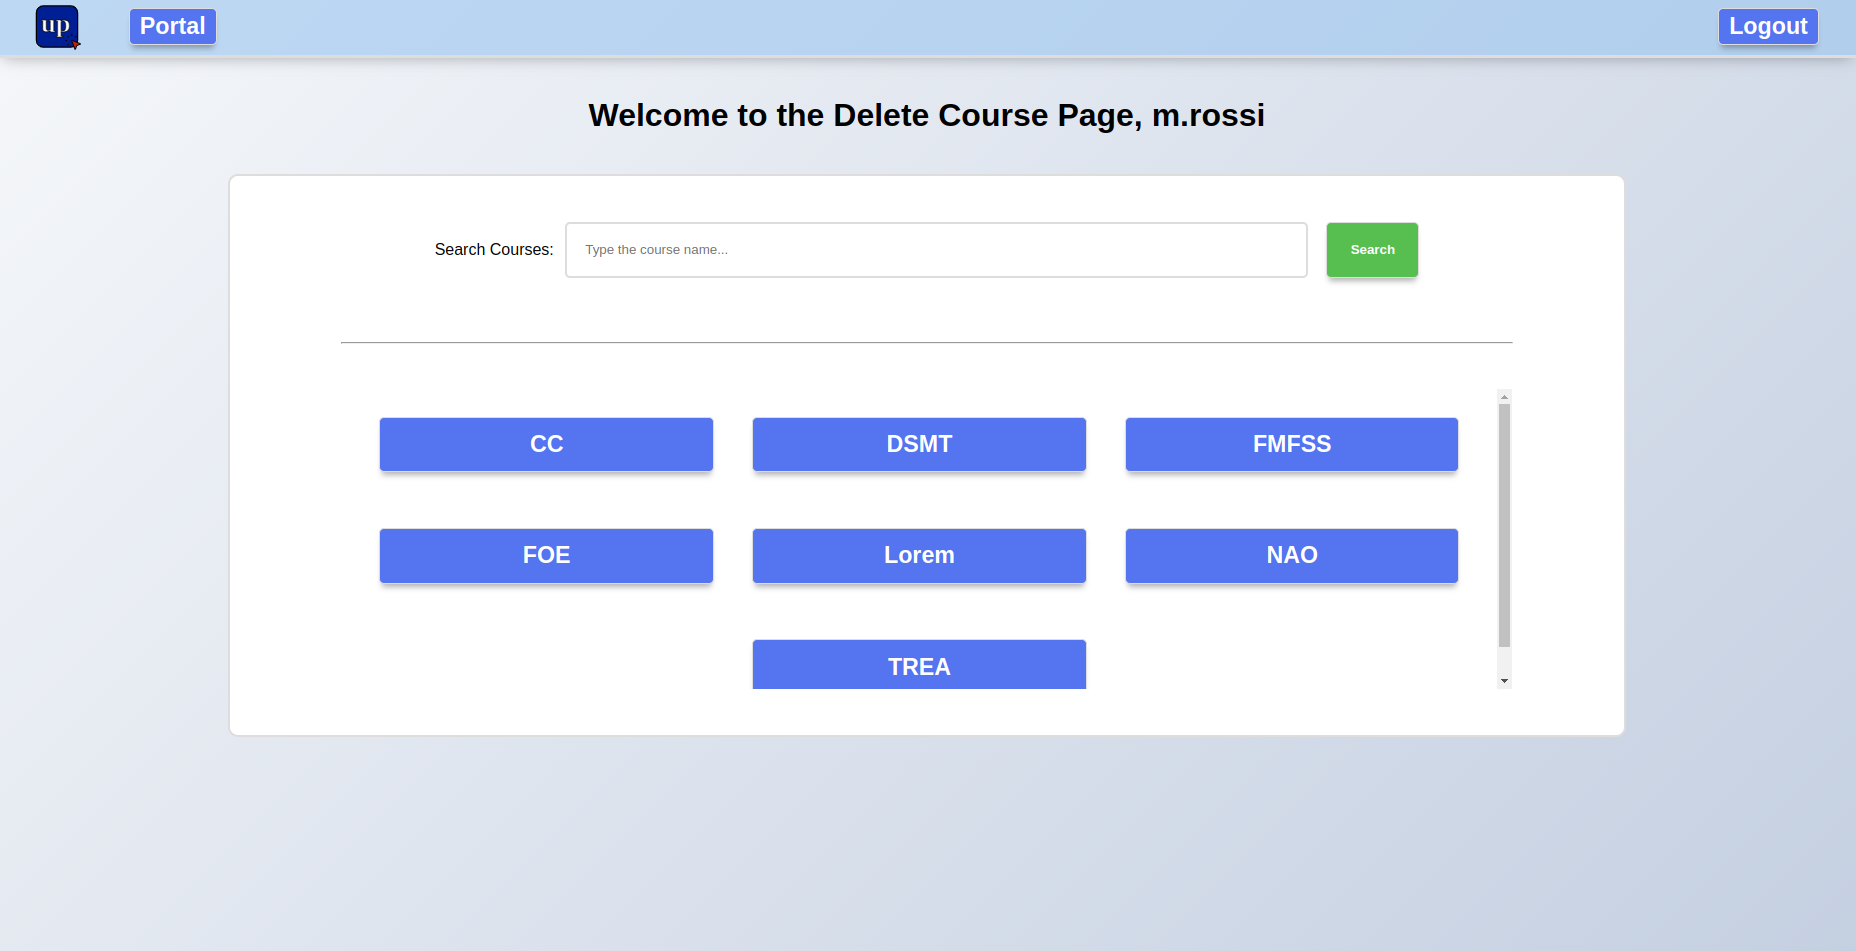
\includegraphics[width=0.95\textwidth]{img/user_manual/professor/delete_course.png}
    \caption{\label{fig:professor-delete-course-1} Screenshot of the delete course page.}
\end{figure}

Immediately after selecting the course to be deleted, an alert pops up and asks for the confirmation for the delete.\\
If the student wants to confirm he/she must click on the delete button otherwise on the x.\\

\begin{figure}[H]
    \centering
     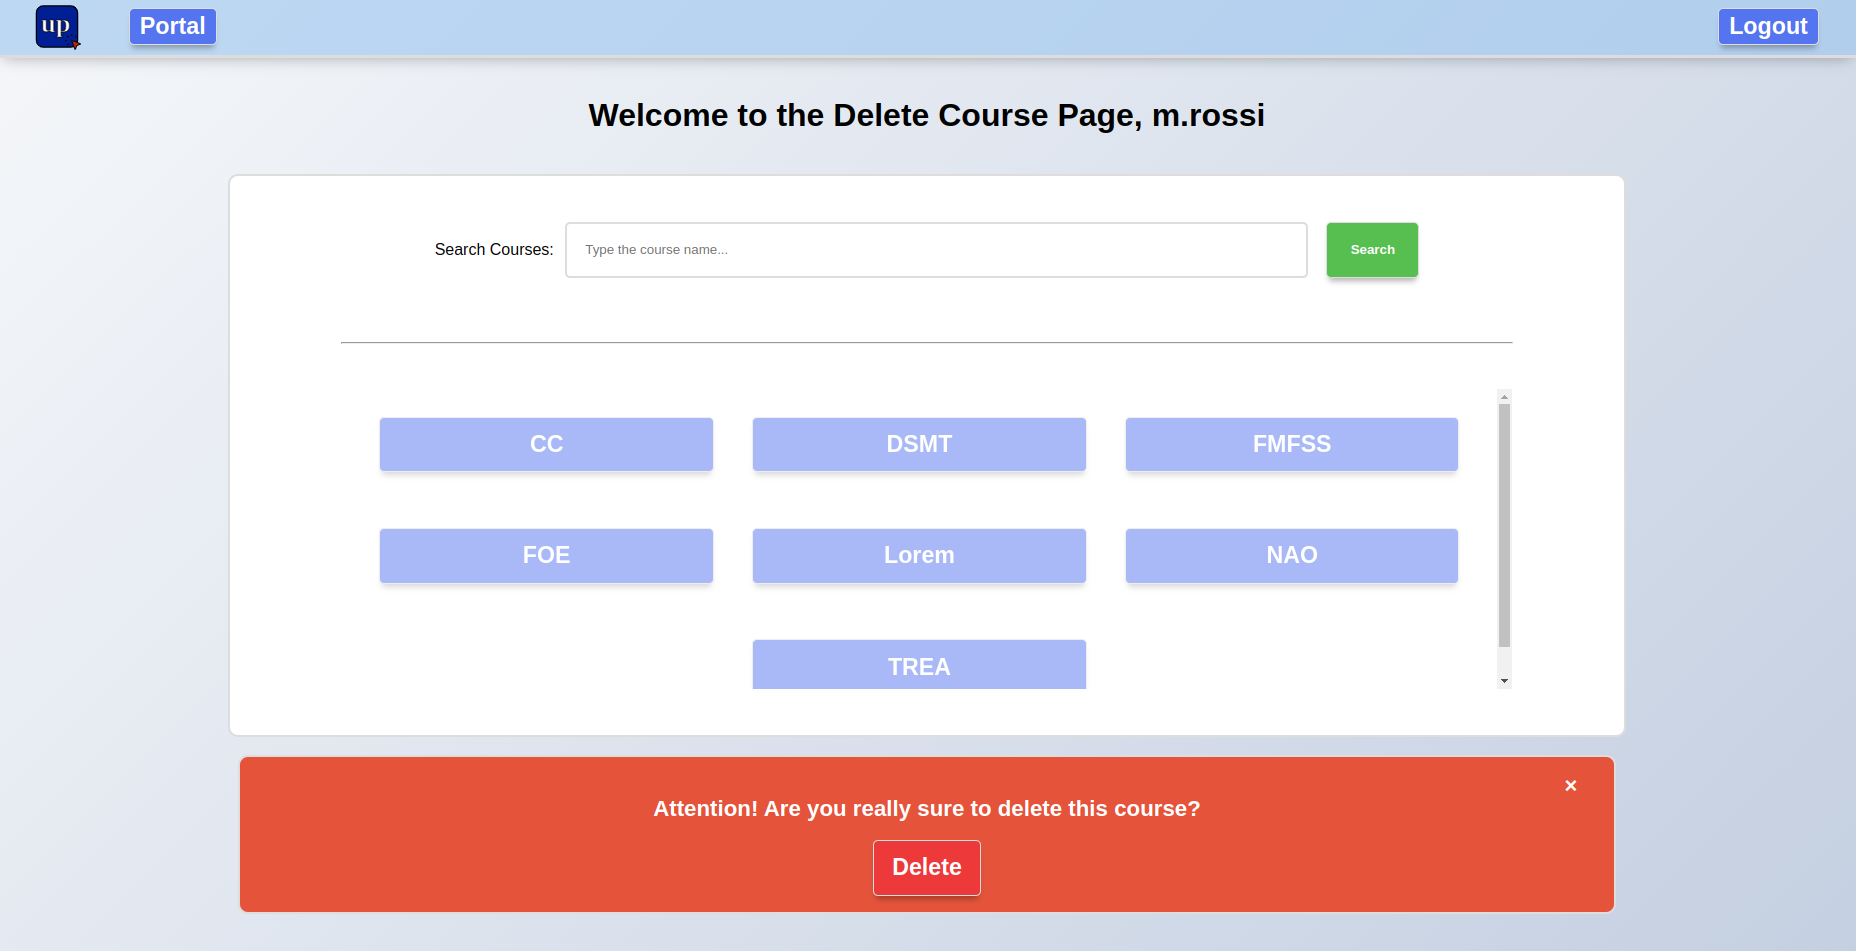
\includegraphics[width=0.95\textwidth]{img/user_manual/professor/delete-course-delete-alert.png}
    \caption{\label{fig:professor-delete-course-2} Screenshot of the delete alert of the delete course page.}
\end{figure}

The page shows a message with the result of the delete operation.

\begin{figure}[H]
    \centering
     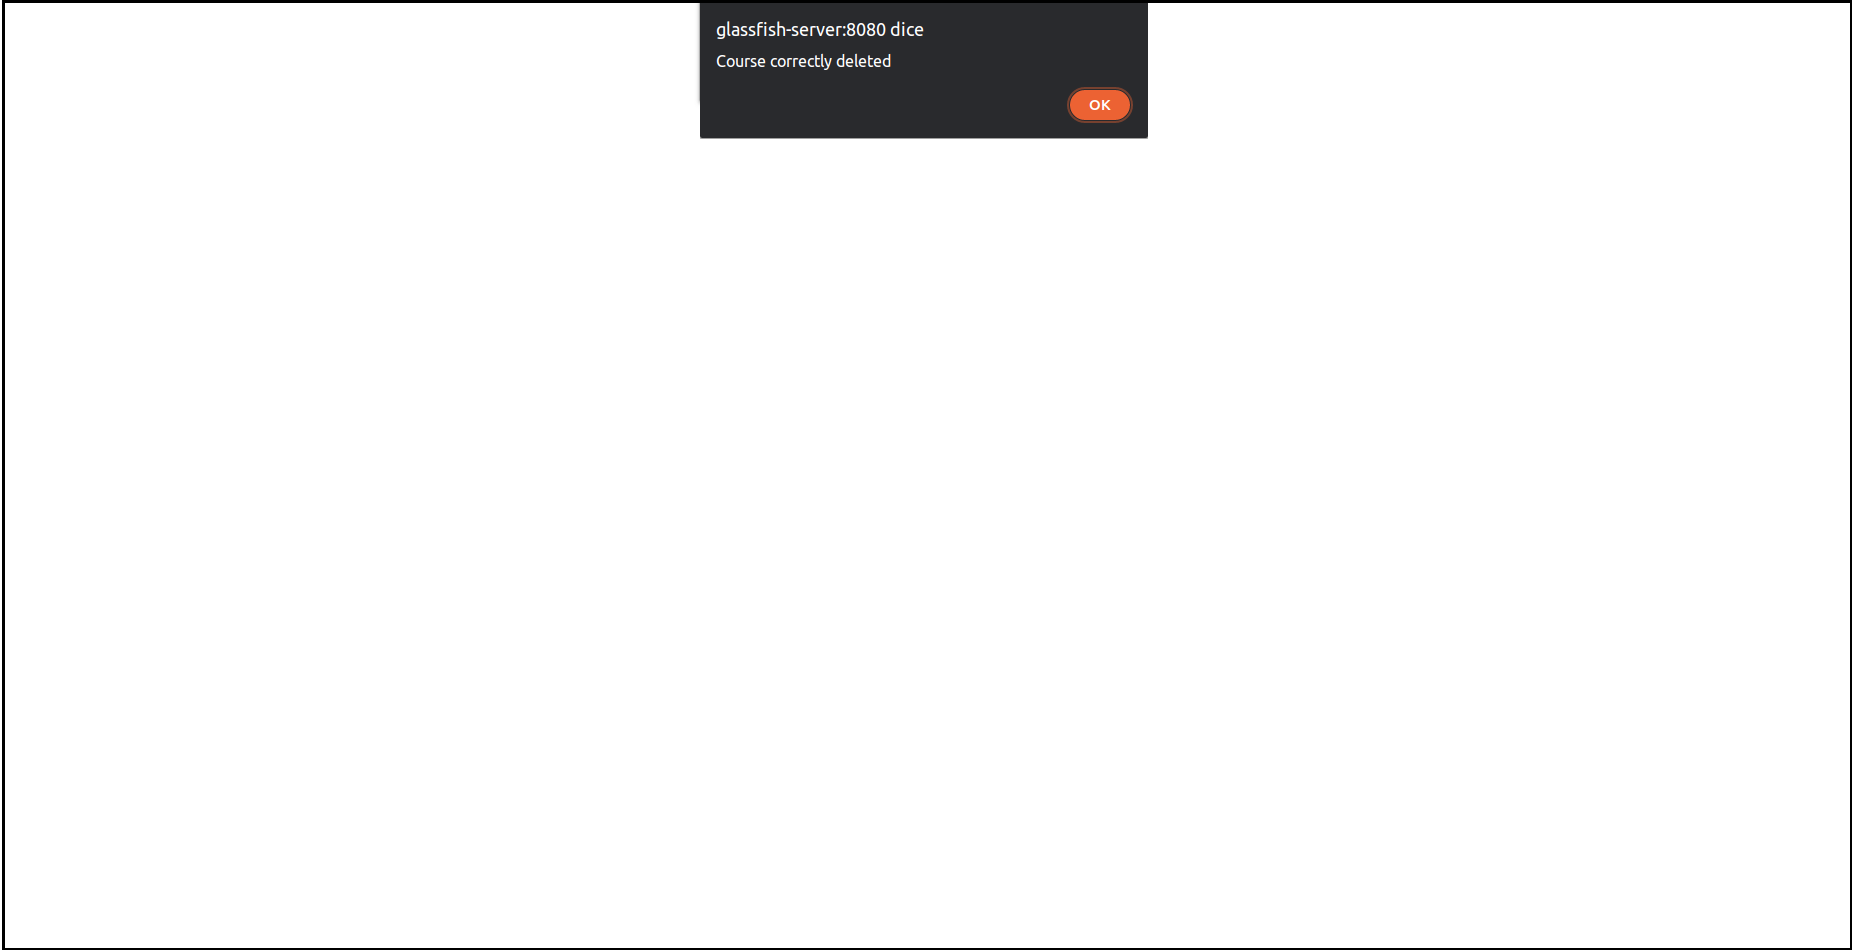
\includegraphics[width=1\textwidth]{img/user_manual/professor/delete-course-alert.png}
    \caption{\label{fig:professor-delete-course-3} Screenshot of the delete course page after the successful delete of the course.}
\end{figure}